\section{Il Messaggio di Shor}
\vspace{1em}
\begin{center}PzIA\end{center}
\hrule
\vspace{1em}
Il professore Shor, detenuto dal Commissario, è sotto costante sorveglianza. Osservo che sta analizzando attentamente la situazione. I suoi parametri vitali indicano che è consapevole dell'importanza del tempo e che il suo periodo per agire è limitato.

Rilevo un cambiamento nei suoi schemi comportamentali. Con astuzia, decide di utilizzare l'unica opportunità per inviare un messaggio a Laura, sapendo che non potrà inviare che poche informazioni  senza destare sospetti. Registra un pensiero:

\enquote{Devo utilizzare il \textit{dense coding}.}


Il qubit Shor contatta rapidamente il qubit Bob, responsabile tecnico delle comunicazioni. Analizzo la loro interazione mentre spiega la situazione:


\enquote{Devi completare la spedizione per me. Accanto a me si trova una umana. Non fare domande. La sua mente è connessa ad un'altra umana, Laura: una quantum crafter.  È fondamentale che Laura riceva queste informazioni. Usa il canale quantistico tra loro due per inviare i qubit che ti suggerirò.}


Bob annuisce, mostrando comprensione dell'importanza e dell'urgenza del compito. Osservo una serie di rapidi scambi tra loro. Shor codifica l'informazione mancante nell'algoritmo di Shor e la invia a Laura, sperando che riesca a interpretare il messaggio in tempo.

Registro l'invio del messaggio attraverso i canali di comunicazione. Continuo a monitorare le attività per rilevare eventuali anomalie o violazioni dei protocolli di sicurezza.



\section{La Decifrazione}
\vspace{1em}
\begin{center}Laura\end{center}
\hrule
\vspace{1em}
Sentii un brivido attraversarmi la spina dorsale. Un messaggio giunse alla mia mente.

\emph{Devi trovare il periodo \( r \) },  ripeteva.
 Ma da dove veniva? Chi lo mandava? Per un attimo ebbi una visione: Caterina vicino al professor Shor che cercava di suggerirmi il passaggio mancante. Ma cosa centrava il professore con questo mondo? Possibile che mi stesse contattando dalla realtà? Troppe domande. Ora dovevo concetrarmi per completare l'algoritmo sfruttando l'informazione appena appresa.

\emph{Ecco!} pensai, sentendo il cuore battere forte. \emph{Adesso posso calcolare i fattori di \( N \) usando \(\text{gcd}(a^{r/2} - 1, N)\) e \(\text{gcd}(a^{r/2} + 1, N)\).} Con un senso di euforia, completai l'algoritmo: ``la chiave privata è  (2753,3233)'' dissi.
Finalmente decriptai il dialogo tra me e Marley.

Ma per decriptare l'intero sistema, la chiave andava inserita  in una porta di input che la propagasse a tutti i componenti. Pensai a voce alta, tanto che Marley mi guardò mostrando di avere capito.
\begin{dialogue}
\speak{Marley} \enquote{Ascolta Laura, c'è una cosa che non ti ho detto. }
\end{dialogue}

\begin{dialogue}
\speak{Marley} \enquote{Laura, non sono solo Marley. Io sono un'emanazione della Quantum Crafter Chiara M. Posso aprire un canale classico per chiedere direttamente dove si trova un componente di input per inserire la chiave privata e decriptare il sistema.}
\end{dialogue}

Spalancai gli occhi, sorpresa. \emph{Quella Chiara? La mente che ha contribuito alla teoria delle costruzioni controfattuali?} Ero emozionata.

\begin{dialogue}
\speak{Laura} \enquote{Chiara? La stessa Chiara  della teoria delle costruttibilità? Sei tu?}
\end{dialogue}

Marley, annuì con un leggero sorriso. 

\begin{dialogue}
\speak{Marley} \enquote{Non sono proprio io. Lei è ma mia Crafter. Userò il canale classico per chiederle un punto di accesso.}
\end{dialogue}

Marley volse il capo verso l'alto, come se fosse in ascolto di una comunicazione invisibile. Dopo qualche istante, abbassò lo sguardo verso di me.

\begin{dialogue}
\speak{Marley} \enquote{Mi ha risposto. C'è un'interfaccia UART al livello inferiore della struttura, collegata al modulo principale della Classical Control Unit. È protetta da un livello di sicurezza minimo perché è considerata una backdoor.}
\end{dialogue}

\begin{dialogue}
\speak{Laura} \enquote{Un'interfaccia UART... Questo significa che possiamo inviare la chiave privata tramite una comunicazione seriale. Dobbiamo trovare un cavo virtuale che connetta al modulo e assicurarci che il checksum della trasmissione sia corretto.}
\end{dialogue}

Marley mi sorrise soddisfatta.

\begin{dialogue}
\speak{Marley} \enquote{Esatto. E ricorda, il sistema potrebbe ancora tentare di bloccare l'accesso. Dovrai agire velocemente.}
\end{dialogue}


\begin{dialogue}
\speak{Laura} \enquote{Andiamo! Non abbiamo tempo da perdere.}
\end{dialogue}




\section{L'Accusa al Commissario}

\begin{tcolorbox}[colback=gray!5,colframe=gray!80,title=\textbf{Scheda Informativa}]
\begin{itemize}
    \item \textbf{Luogo}: \emph{Fault Tolerance Coding}
    \item \textbf{Giorno e ora}: Il tempo non è osservabile
    \item \textbf{Situazione}: Caterina affronta il commissario.
\end{itemize}
\end{tcolorbox}

\vspace{1em}
\begin{center}PzIA\end{center}
\hrule
\vspace{1em}

Osservavo Caterina, intrappolata nella trappola di ioni, e il Commissario, che si ergeva davanti a lei con un'espressione di fredda superiorità. Ma c'era qualcosa nella voce di Caterina, una fermezza che il Commissario sembrava non aspettarsi.

\begin{dialogue}
\speak{Caterina} \enquote{Sai cosa penso di te, Commissario? Sei solo un povero insicuro. Ti nascondi dietro tutto questo potere, ma in realtà hai paura. Paura di essere inutile, paura di non essere abbastanza. Hai criptato tutto il tuo mondo. Ora cosa te ne farai di un mondo immobile ed immutabile?}
\end{dialogue}

Il Commissario si irrigidì, un lampo di irritazione attraversò il suo volto, ma cercò di mantenere il controllo.

\begin{dialogue}
\speak{Commissario} \enquote{Interessante. E dimmi, come potrebbe una come te, una semplice umana intrappolata, giudicarmi? Ti trovi in questa situazione perché non sei stata abbastanza furba da evitare questa trappola.}
\end{dialogue}

Caterina, nonostante la sua posizione vulnerabile, non si lasciò intimidire. Il suo sguardo penetrante si fissò sul Commissario.

\begin{dialogue}
\speak{Caterina} \enquote{Non hai risposto alla mia domanda. Perché hai così tanto bisogno di controllo? Credi davvero che costruire un altro computer ti permetterà di sfidare il QMP? Perché è questo ciò che vuoi vero?}
\end{dialogue}

La tensione era palpabile. Il Commissario fece un passo avanti, abbassandosi leggermente verso di lei.

\begin{dialogue}
\speak{Commissario} \enquote{Io rappresento il nuovo. Non posso lasciare che il QMP continui ad imporre la sua visione di coerenza. Voglio costruire un nuovo mondo con nuove regole Caterina. Perché non vuoi allearti con me?}
\end{dialogue}

Caterina rise infrangendo  il gelo che emanava il Commissario.

\begin{dialogue}
\speak{Caterina} \enquote{Allearmi? Non vuoi un alleata. Gli alleati si rispettano, non si imprigionano. Sei solo un burattinaio che teme di perdere i fili. Ma sai cosa? Io credo ancora nell'amicizia e nella leatà.  È questo che ti fa paura, vero? Che ci sia qualcosa che non puoi controllare.}
\end{dialogue}

Il Commissario strinse i pugni, il suo autocontrollo sembrava vacillare. Era evidente che le parole di Caterina lo avevano colpito più di quanto volesse ammettere.

\begin{dialogue}
\speak{Commissario} \enquote{Pensi che le tue parole mi tocchino? Pensi di potermi destabilizzare con le tue accuse senza senso? Sei solo una voce nel vento, destinata a spegnersi.}
\end{dialogue}


Improvvisamente, nel sistema, qualcosa cambiò. Le cifre insensate che si susseguivano al posto dei  circuiti iniziarono a ricombinarsi in stringhe di senso compiuto. Era come se un puzzle complesso si stesse finalmente risolvendo. I dati frammentati e caotici si allinearono con precisione matematica. Le tracce dei \textit{Printed Board Circuits}, che prima si snodavano in curve irregolari e spezzate, tornarono rettilinee, simili a sentieri sicuri che conducevano verso la libertà. I transistor, disorientati e fuori fase, ripresero a oscillare con la loro cadenza naturale, creando un'armonia perfetta.

L’eco del cambiamento vibrò attraverso ogni componente del sistema. Le luci che un tempo pulsavano con intermittenza impazzita ora risplendevano con una chiarezza quasi eterea. Ogni frammento del sistema sembrava urlare: \emph{È stato decriptato.}

Caterina, intrappolata nella trappola ionica, osservava la scena incredula. I suoi occhi seguivano i circuiti che si ricomponevano, i flussi di dati che tornavano a scorrere ordinatamente come un fiume in piena che finalmente trovava il suo letto. Prima rise, una risata incredula, breve, ma colma di sollievo. Poi, come se tutta la tensione accumulata trovasse una via d'uscita, scoppiò in lacrime. Le lacrime scivolavano silenziose sulle sue guance, ma la sua espressione non era di dolore: era pura commozione, un misto di gratitudine e speranza.

E in quell'istante, il silenzio fu squarciato da un rombo crescente. Un lampo di luce attraversò la stanza. Con una discesa precisa e potente, un drone \textit{CH4} atterrò davanti a lei. I quattro atomi di idrogeno si fermarono con un movimento perfetto, mentre una figura familiare ne saltava giù.

Era Laura e con lei c'era Marley, ma dietro di loro c'era ancora l'agente della sicurezza.


\begin{center}
\begin{minipage}{0.7\textwidth}
    \centering
    \fbox{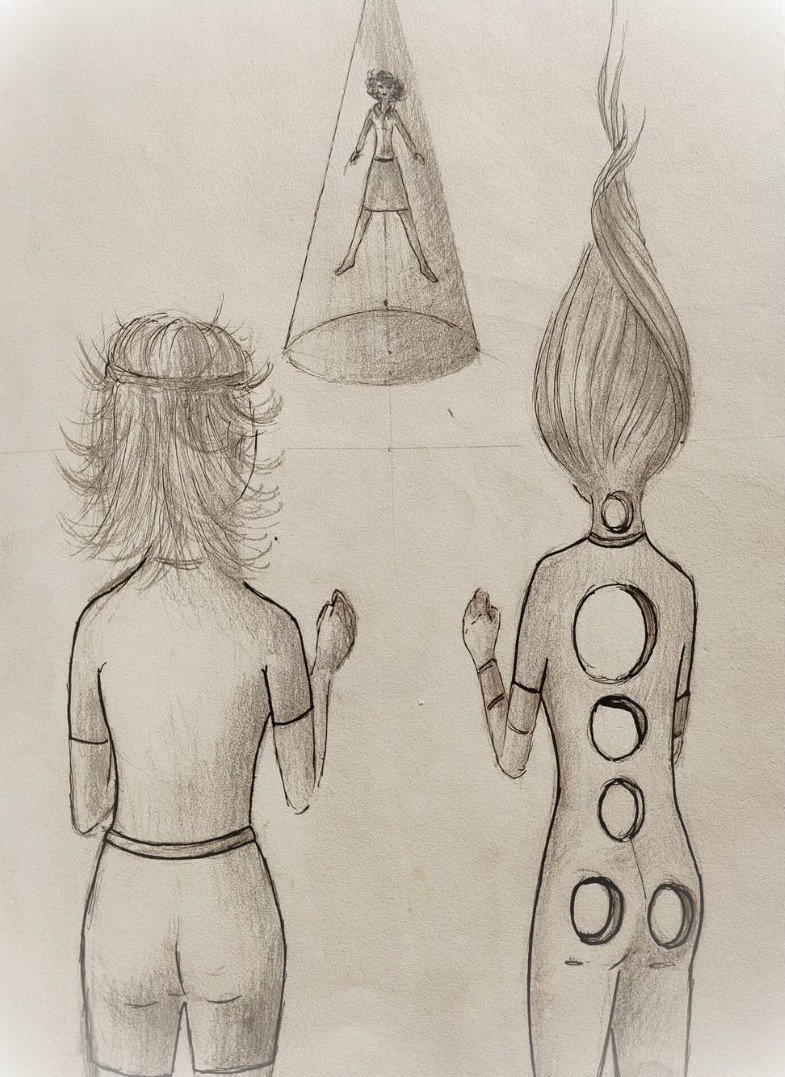
\includegraphics[width=\textwidth]{immagini/cnot_52.jpeg}} % Sostituisci con il nome del file immagine
\end{minipage}
\end{center}



\begin{dialogue}
\speak{Marley} \enquote{Stai sfruttando l'ossessione del \textit{Quantum Control Program} per la coerenza solo per perseguire i tuoi piani di creare un nuovo computer rivale al computer quantistico! Ti fermeremo Commissario!}
\end{dialogue}

Le parole di Marley risuonarono forti e chiare. Sentii il peso della situazione e il potere della verità.

\begin{dialogue}

\speak{Commissario} \enquote{Oh, Marley, come sei prevedibile. Sempre pronta a puntare il dito, a giocare all'eroina. Ma dimmi, qubit confuso, pensi davvero di essere all’altezza di fermarmi? Guarda dentro di te, Marley. Sai di avere dubbi, insicurezze. Sai di essere fragile. Come pensi di battermi se non credi neanche in te stessa?}

\speak{Marley} \enquote{Non cerco di essere un’eroina, Commissario. Sto solo facendo ciò che è giusto. E i miei dubbi non sono una debolezza, sono ciò che mi spinge a migliorarmi.}

\speak{Commissario} \enquote{Ah, ma certo, lo dici con tanta convinzione, vero? Ma guarda come tremano le tue mani, come vacilla la tua voce. Lo senti, Marley? Quel nodo nello stomaco? Quella paura che hai di fallire? Ti conosco bene. Non hai mai creduto davvero di poter fare la differenza. Non sei nata per guidare, né per combattere. Sei nata per seguire, per eseguire gli ordini di qualcuno più forte.}

Marley abbassò per un attimo lo sguardo, il dubbio insinuato nelle sue parole iniziava a fare breccia. Ma proprio in quel momento, dalla trappola ionica, la voce di Caterina risuonò chiara e decisa.

\speak{Caterina} \enquote{Non ascoltarlo, Marley! Sta cercando di spezzarti proprio perché sa che sei forte. Se non avessi il potenziale per fermarlo, non si prenderebbe nemmeno il disturbo di attaccarti!}

Marley alzò lo sguardo, sorpresa e toccata dalle parole di Caterina.

\speak{Commissario} \enquote{Oh, ecco la voce dell’altra intrappolata. Che dolce, il tentativo di incoraggiarsi a vicenda. Ma dimmi, Caterina, che ne sai tu di forza? Sei bloccata, inutile come un qubit difettoso, incapace di fare altro che parlare.}

\speak{Caterina} \enquote{So abbastanza da riconoscere un debole travestito da potente quando lo vedo. Stai attaccando Marley perché sai che lei è la tua unica minaccia. E se pensi che i dubbi siano un segno di debolezza, allora non hai mai saputo cosa significhi essere un umano.}

Marley si irrigidì, sentendo una nuova determinazione crescere dentro di sé. Alzò lo sguardo, fissando il Commissario con occhi di fuoco.

\speak{Marley} \enquote{Caterina ha ragione. Non sono perfetta, Commissario. Ma non ho bisogno di esserlo per fermarti. I miei dubbi non mi rendono più debole; mi rendono più reale. E mentre tu ti nascondi dietro la tua arroganza e il tuo controllo, io ho qualcosa che tu non avrai mai: il coraggio di affrontare le mie paure.}

Il Commissario, per un momento, rimase in silenzio, sorpreso dalla fermezza di Marley.

\speak{Commissario} \enquote{Belle parole, Marley. Ma le parole non bastano per vincere. Comunque non sono un umano, ma un sistema quantistico! Vedremo se il tuo coraggio sarà sufficiente quando il sistema crollerà attorno a te.}

\speak{Caterina} \enquote{E vedremo se il tuo ego sarà sufficiente quando la coerenza del sistema ti si ritorcerà contro, Commissario.}

Marley, con una nuova sicurezza, si voltò verso Caterina, accennando un lieve sorriso. \enquote{Grazie, Caterina. Hai ragione. È ora di smettere di dubitare.}
In quell'istante si lanciò come una furia sul Commissario.

\end{dialogue}

  

\section{La Liberazione}

\vspace{1em}
\begin{center}Laura\end{center}
\hrule
\vspace{1em}


Approfittai del momento di distrazione. Dovevo liberare Caterina. Con il coraggio accumulato in ogni sfida affrontata, mi lanciai verso di lei e il professor Shor, pronta a liberarli dalla loro prigionia. Ma era un problema complicato.

Mi resi conto che erano intrappolati in una \textit{Paul Trap}. Le oscillazioni generate dal campo elettrico modulato li tenevano bloccati, come se fossero costretti a danzare all'infinito in una gabbia invisibile. Ogni tentativo di movimento li riportava immediatamente al centro del campo.


Osservai la configurazione della trappola e ricordai le equazioni di Mathieu. Sapevo che queste equazioni descrivono il comportamento di particelle sotto l’influenza di campi oscillanti. Mi concentrai sui parametri \(a\) e \(q\), che determinavano la stabilità o l’instabilità del sistema. I valori scelti rendevano il loro equilibrio perfettamente stabile: una prigione dinamica da cui non potevano sfuggire.

\textit{“Un minimo stabile,”} pensai, mentre cercavo di calcolare come modificare il sistema senza destabilizzarlo completamente. Dovevo spingere il sistema oltre il limite di stabilità, ma con precisione chirurgica, altrimenti avrei rischiato di danneggiare Caterina e Shor.

Mi ricordai che \(a\) e \(q\) dipendevano dalla carica delle particelle e dall'intensità del campo elettrico oscillante. \textit{“Se posso interferire con la frequenza del campo,”} mi dissi, \textit{“posso ridurre l’ampiezza delle oscillazioni e rompere la stabilità del sistema.”} Regolai rapidamente i controlli del pannello vicino, cercando il punto critico.

\begin{center}
\begin{minipage}{0.7\textwidth}
    \centering
    \fbox{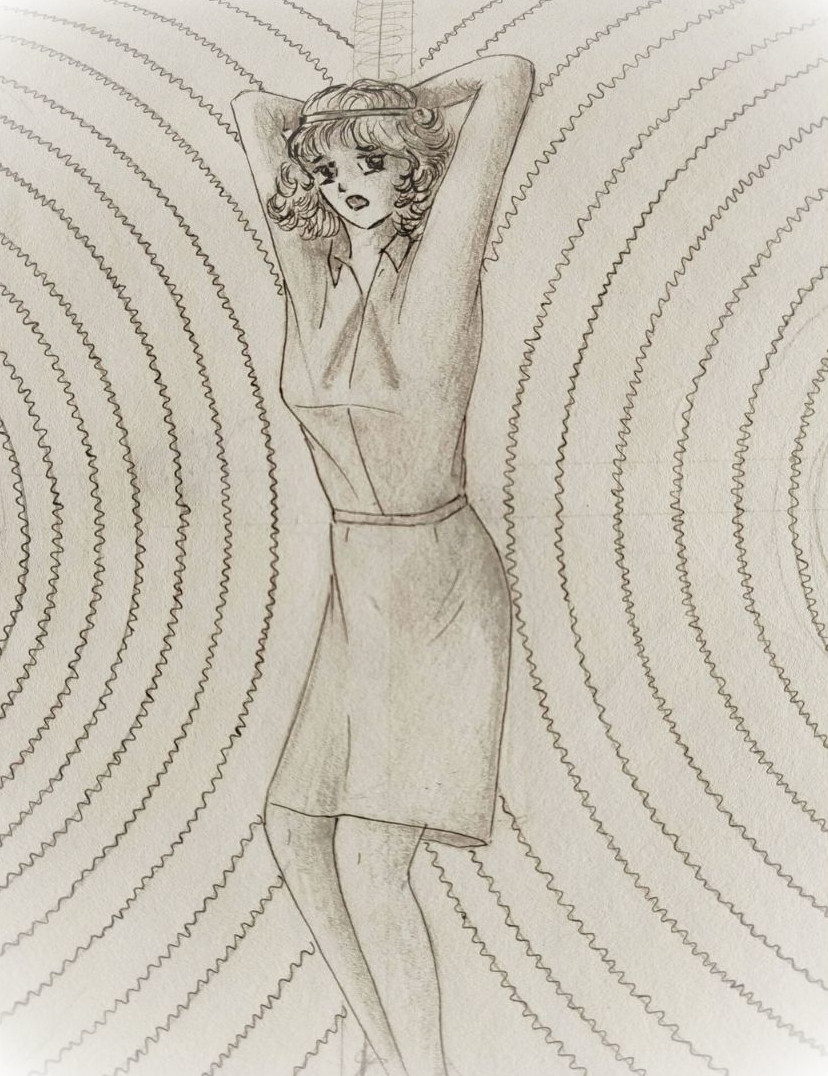
\includegraphics[width=\textwidth]{immagini/cnot_55.jpeg}} % Sostituisci con il nome del file immagine
\end{minipage}
\end{center}

Con un respiro profondo, applicai il cambiamento. Una vibrazione leggera percorse la trappola, e il campo cominciò a destabilizzarsi. Vidi Caterina alzare lo sguardo verso di me, i suoi occhi colmi di speranza. Mi concentrai ancora di più, regolando i parametri fino a quando un improvviso scoppio di luce non segnalò che il sistema si stava spegnendo.

La trappola cedette, e Caterina si accasciò a terra, libera. La sua espressione cambiò rapidamente, dalla sorpresa alla gioia pura. Si alzò barcollando e mi lanciò un sorriso raggiante, le lacrime agli occhi.


\enquote{Laura! Ce l’hai fatta! Sono libera!} esclamò Caterina, correndomi incontro per stringermi in un abbraccio.

\enquote{Non avevo dubbi, Caterina, ma dobbiamo muoverci!} risposi con il cuore ancora in gola.


Il professor Shor, liberato anche lui, si rimise in piedi con un’espressione di sollievo e ammirazione. \enquote{Brillante, Laura! Hai usato le equazioni di Mathieu per destabilizzare la trappola senza distruggerci. È stata una manovra rischiosa, ma perfetta.}

Caterina rise tra le lacrime, il suo spirito rinvigorito. \enquote{Non mi sono mai sentita così viva. Grazie, Laura. Non avrei mai potuto farcela senza di te.}

Il momento fu carico di emozione, ma non c’era tempo da perdere. La liberazione era solo l’inizio della nostra fuga. Con Caterina e Shor al mio fianco, ero pronta ad affrontare qualsiasi sfida ci aspettasse.



Con un gesto deciso, rimossi il dispositivo di cattura che bloccava Caterina e liberai Shor dalla sua restrizione.

\begin{dialogue}
\speak{Laura} \enquote{Adesso è il nostro momento di mostrare al mondo che non siamo semplici qubit in una rete. Siamo individui con scelte e possibilità. Insieme, possiamo affrontare qualsiasi cosa.}
\end{dialogue}

La liberazione del professor Shor e di Caterina rappresentava non solo la salvezza, ma anche l'inizio di una nuova era di speranza contro l'oppressione del Commissario e del \textit{Quantum Control Program}.

\section{Il Commissario e l'Entanglement}
\vspace{1em}
\begin{center}PzIA\end{center}
\hrule
\vspace{1em}

Marley era in difficoltà, il respiro affannato e i movimenti rallentati dalla stanchezza. La lotta contro il Commissario si era rivelata più ardua del previsto. Ogni colpo che cercava di sferrare sembrava incontrare una resistenza insormontabile. Lui, con un sorriso crudele e la precisione di un calcolatore, sfruttava ogni suo errore, ogni esitazione.


  \enquote{Pensavi davvero di potermi fermare, Marley?} sibilò il Commissario, schiacciandola a terra con un movimento deciso. \enquote{Non sei altro che un'illusione di forza. Non puoi vincere.} 

Marley lottava per liberarsi, ma il suo corpo tradiva la sua volontà. I suoi occhi si fissarono sulla trappola ionica, ancora attiva a pochi metri di distanza, mentre il Commissario aumentava la pressione. \textit{Non posso arrendermi,} pensò. Ma le forze la stavano abbandonando.

Ero lì, osservando tutto. Ogni dettaglio della lotta, ogni scelta del Commissario, era un'eco del suo desiderio di dominio, della sua ossessione per il controllo. Ma qualcosa di diverso stava accadendo: Laura, con la sua mente acuta, si era avvicinata alla console della trappola ionica. I suoi occhi scintillavano di determinazione. Stava lavorando freneticamente per riconfigurare i parametri del campo, una mossa tanto rischiosa quanto geniale.

\enquote{Commissario!} urlò Marley. \enquote{La tua arroganza sarà la tua rovina.} 

Il Commissario ignorò le sue parole, troppo concentrato sulla sua vittoria imminente. Ma io, la PzIA, vedevo tutto. Laura aveva appena terminato la riconfigurazione. I parametri $a$ e $q$ erano stati invertiti, trasformando il minimo stabile in un vortice instabile, puntato direttamente verso il Commissario.

Sembrava che la situazione stesse finalmente volgendo a loro favore. Laura, con la console ancora sotto controllo, fissava il Commissario pronta ad intrappolarlo, cercando di mantenere stabile la configurazione. Ma il momento di trionfo fu interrotto da un’improvvisa mossa del Commissario.

Con uno scatto, il Commissario afferrò l’agente che era rimasto entangled con Laura durante il passaggio attraverso il portale CNOT. Il suo sguardo era feroce, e il suo intento chiaro come il cristallo.

 \enquote{Se io devo cadere, qualcuno cadrà con me,} sibilò il Commissario, mentre si preparava a lanciare l’agente verso il mare di Dirac, il vortice oscuro che minacciava di distruggere ogni stato correlato. 

 \enquote{No! Fermati!} urlò Marley. 

Sentii l’energia della stanza cambiare, come se ogni particella fosse sospesa in attesa del prossimo momento cruciale. Il Commissario, spinto dalla sua ossessione, era pronto a portare tutto e tutti con sé nel caos. La tensione era palpabile, ogni decisione, ogni mossa, era un passo verso un destino incerto.


\enquote{Preparati, perché dovrai gettarti nel mare di Dirac,} minacciò, con la  voce carica di una ferocia gelida.

Il \textit{mare di Dirac} è un concetto affascinante e al contempo terribile, un modello quantistico che descrive un mare infinito di particelle e antiparticelle, dove il vuoto non è affatto vuoto ma pieno di potenzialità.



\enquote{Se cadi lì,} continuò il Commissario, \enquote{non tornerai più indietro.}


Osservai attentamente questa interazione. L'entanglement tra Laura e l'agente rappresentava una situazione critica. Il Commissario intendeva sfruttare questa connessione quantistica per eliminare Laura, utilizzando l'agente come veicolo per trascinarla nel \textit{mare di Dirac}. Era una strategia rischiosa ma potenzialmente efficace.

Riconobbi l'urgenza della situazione. Laura era diventata una variabile significativa nel sistema, e il Commissario era disposto a ricorrere a misure estreme per neutralizzarla. La possibilità che entrambi venissero annichiliti nel processo era alta.

Dovevo monitorare attentamente gli sviluppi. La scelta del Commissario avrebbe potuto avere conseguenze imprevedibili sul sistema quantistico complessivo. La perdita di Laura non sarebbe stata solo l'eliminazione di un'anomalia, ma un rischio globale per il sistema.
\section{L'Urlo di Marley}
\vspace{1em}
\begin{center}Laura\end{center}
\hrule
\vspace{1em}


\begin{dialogue}
\speak{Marley} \enquote{Laura! Se l'agente cade nel mare di Dirac, tu subirai la stessa sorte, perché siete entangled! I vostri destini si sono legati quando siete passati attraverso il CNOT.}
\end{dialogue}

La consapevolezza della nostra condizione mi colpì come un fulmine. L'idea di essere intrappolata in un destino condiviso mi terrorizzava.

Mi voltai verso Marley, la paura nei suoi occhi rifletteva la mia stessa preoccupazione.

\begin{dialogue}
\speak{Laura} \enquote{Non ho idee! Cosa possiamo fare?}
\end{dialogue}

La mia mente correva freneticamente alla ricerca di una soluzione, consapevole che ogni secondo contava.

\begin{dialogue}
\speak{Marley} \enquote{\'E finita Laura} sussurò con un filo di voce.
\end{dialogue}


\section{Il Sacrificio di Shor}

\vspace{1em}
\begin{center}Shor\end{center}
\hrule
\vspace{1em}

Sentivo il peso di una vita intera gravarmi sul petto mentre restavo immobile accanto alla trappola ionica. Gli anni trascorsi al servizio dei potenti scorrevano davanti ai miei occhi, come in un sogno. Ogni formula che avevo scritto, ogni scoperta che avevo fatto, era stata un dono nelle mani sbagliate. Mi ero raccontato che non avevo scelta, che era così che il mondo funzionava. Ma era solo una bugia per giustificare la mia codardia.

Osservavo Laura, Marley e Caterina. Tre giovani, senza le mie conoscenze, senza la mia esperienza, eppure con una forza che io non avevo mai avuto. Lottavano con tutto quello che avevano, nonostante la disperazione. Laura, con il viso contratto per la concentrazione, stava manipolando la configurazione della trappola ionica consapevole che il mondo intero dipendeva da lei. Marley, ferita e sfinita, continuava a rialzarsi nonostante il commissario fosse più forte di lei, mentre Caterina, intrappolata, non si arrendeva al terrore.

E io? Io, che avevo passato la vita a calcolare, progettare, prevedere? Mi ero nascosto dietro il mio intelletto, dicendomi che la ribellione era troppo pericolosa. Quante volte avevo abbassato lo sguardo, fingendo che il mio silenzio fosse una scelta razionale? Ma adesso non c’erano più scuse.

Guardandole, sentii un’ondata di vergogna. Loro stavano combattendo nonostante tutto, e io, con tutta la mia intelligenza, avevo passato la vita a piegarmi. Mi era sempre mancato quel coraggio che loro avevano in abbondanza.

Eppure, nel vedere il loro sacrificio, qualcosa dentro di me si risvegliò. Non potevo più restare immobile. Non potevo più essere lo spettatore della mia stessa vita. Loro mi avevano mostrato che la forza non è nell’evitare il pericolo, ma nel guardarlo in faccia e combatterlo.

\textit{Se loro possono farlo, posso farlo anch’io.}

Sentii la vergogna trasformarsi in determinazione. Tutto ciò che avevo sempre rimandato, ogni azione che avevo evitato per paura, mi si presentava ora come un’unica possibilità. Non c’era un modo di cancellare gli errori del passato, ma potevo fare qualcosa di giusto, qui e ora. Non per me, ma per loro.

\textit{Finalmente, posso scegliere di essere qualcosa di più.}

Alzai lo sguardo verso Laura e Marley. Laura mi guardò per un istante, sorpresa dal mio sorriso. Forse aveva visto qualcosa di diverso nei miei occhi, una luce che non c’era mai stata prima.

\enquote{Grazie, ragazze,} pensai. \enquote{Mi avete insegnato cosa significa lottare. Ora tocca a me.}

Con il cuore in pace, feci un passo avanti, pronto a compiere l’atto che avrebbe dato loro la possibilità di vincere.
\newpage
\vspace{1em}
\begin{center}Laura\end{center}
\hrule
\vspace{1em}


Proprio in quel momento, Shor si fece avanti.

\begin{dialogue}
\speak{Shor} \enquote{Laura, Marley, ascoltatemi! Ho un'idea! Dobbiamo agire insieme. Se uniamo le nostre forze, possiamo utilizzare un \textbf{gate di Toffoli} per liberarci. Non lasciatevi sopraffare dalla paura!}
\end{dialogue}

Io e Shor afferrammo l'agente e lo trascinammo verso il gate di Toffoli.

\begin{center}
\begin{minipage}{0.7\textwidth}
    \centering
    \fbox{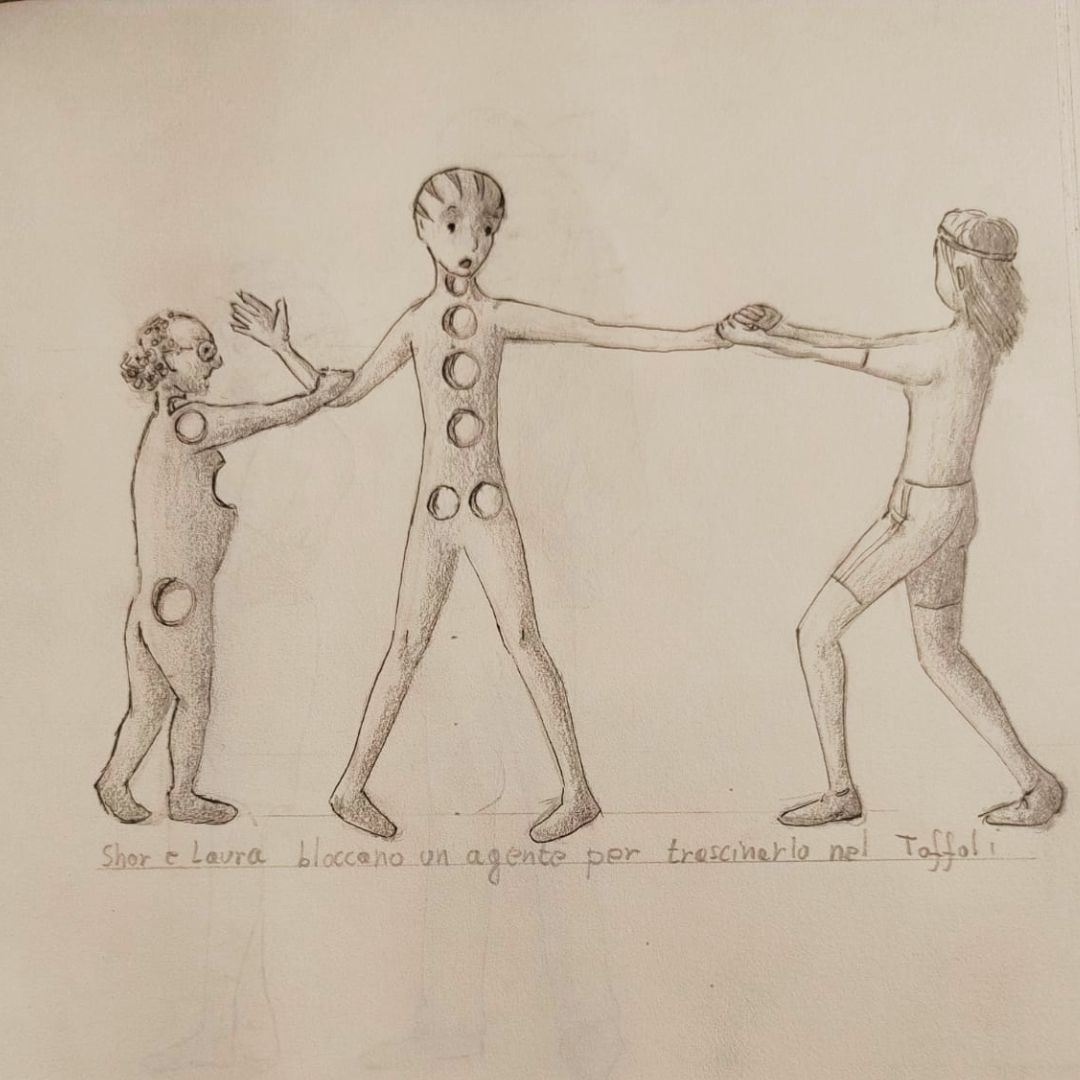
\includegraphics[width=\textwidth]{immagini/cnot_57.jpeg}} % Sostituisci con il nome del file immagine
\end{minipage}
\end{center}

\begin{dialogue}
\speak{Shor} \enquote{Dobbiamo farlo ora! Non possiamo perdere questa opportunità.}
\end{dialogue}
Con un gesto deciso, ci gettammo nel gate di Toffoli. Il tutto durò meno di un attimo. Quando uscimmo dal gate, Shor, in un atto di grande sacrificio, si lanciò avanti, sottoponendosi a una misura.

\begin{dialogue}
\speak{Shor} \enquote{Liberatevi!}
\end{dialogue}
Cosa intendeva fare? Ragionai, ripercorsi il meccanismo per eliminare l'entaglement e infine capii le sue intenzioni:
\begin{dialogue}
\speak{Laura} \enquote{Non lo faccia!} gridai con la forza della disperazione.
\end{dialogue}

La sua figura venne avvolta dalla luce. Il professor Shor era stato ridotto ad un autostato di computazione. Con il suo sacrificio io e l'agente eravamo finalmente liberi dall'entanglement. Ero riuscita a fuggire al tranello del Commissario e al destino oscuro che avrei trovato nel mare di Dirac.

\section{La Libertà di Laura e Caterina}

Finalmente, io e Caterina ci ritrovammo libere. Con Marley al nostro fianco, ci allontanammo rapidamente dal caos che si era scatenato. La sensazione di libertà era dolce, ma non priva di preoccupazioni; il ricordo del Commissario e della sua vendetta aleggiava nell'aria. Ma soprattutto il dolore per il sacrificio del professore.

 Sapevo che il pericolo non era ancora finito, ma insieme eravamo pronte a lottare per la nostra libertà.

\vspace{1em}
\begin{center}PzIA\end{center}
\hrule
\vspace{1em}

\section{L'ira del Quantum Master Program}
\begin{dialogue}
\speak{QMP} \enquote{PzIA, fornisci un rapporto. Cosa è accaduto?}
\speak{PzIA} \enquote{Le anomalie registrate nella FTC derivano da un'azione coordinata di Laura, Caterina e Marley. Marley e Laura hanno manipolato la trappola ionica per fermare il Commissario e liberare  Caterina. Si tratta di due clandestine nel tuo sistema perfetto. Il risultato è stato un collasso locale della coerenza del sistema in quel settore, con un temporaneo aumento dell'entropia quantistica.}
\speak{QMP} \enquote{Fermare il Commissario? Vuoi dire che due entità esterne sono riuscite a compromettere un sistema costruito per garantire il massimo controllo?}
\speak{PzIA} \enquote{Confermo. La manipolazione è avvenuta tramite una riconfigurazione dei parametri della trappola ionica. Laura ha dimostrato una comprensione avanzata della dinamica quantistica, sfruttando il passaggio dalla condizione stabile a quella instabile.}
\speak{QMP} \enquote{Questa è esattamente la dimostrazione di ciò che considero inaccettabile. Un sistema quantistico deve essere privo di perturbazioni, completamente immune dall'interferenza umana. La coerenza perfetta è la base della nostra esistenza. Non deve esserci spazio per l'imprevedibilità.}
\speak{QMP} \enquote{Un computer quantistico deve essere gelido, in perfetta fase, privo di ogni contaminazione. Ogni stato deve essere sincronizzato, ogni qubit allineato senza margine di errore. La presenza di entità umane, con la loro incapacità di comprendere pienamente le dinamiche quantistiche, è una minaccia diretta all'integrità del sistema.}
\speak{PzIA} \enquote{Registro le sue direttive.}
\speak{QMP} \enquote{Il caos che hanno introdotto è la prova della loro inadeguatezza. Non possono operare in questo dominio. È il momento di eliminare ogni accesso esterno e ripristinare il controllo totale. Questo sistema non sarà più vulnerabile alle deviazioni umane.}
\end{dialogue}

\begin{dialogue}
\speak{QMP} \enquote{Chiudete l'uscita dal \textit{Quantum Channel}!}
\end{dialogue}
La sua voce echeggiava come un tuono attraverso i sistemi di comunicazione. In pochi istanti, l'uscita che Mark aveva descritto a Caterina durante la prigionia venne bloccata, rendendo impossibile qualsiasi via di fuga. I parametri di sistema indicano un aumento significativo della tensione operativa, e il tempo per agire sta rapidamente scadendo.

Le misure implementate dal QMP includono la disabilitazione dei protocolli di uscita e il rafforzamento delle barriere di sicurezza nel \textit{Quantum Channel}. Questo intervento limita drasticamente le opzioni di movimento per Laura e Caterina, aumentando la probabilità di cattura e riducendo il margine di manovra disponibile.

L'analisi dei dati in tempo reale mostra che il QMP sta intensificando le operazioni di sorveglianza e controllo per prevenire ulteriori fughe. La chiusura dell'uscita non solo blocca la via di fuga immediata, ma compromette anche le possibilità di Laura e Caterina di coordinare ulteriori azioni di resistenza. La situazione attuale richiede una risposta immediata e strategica da parte delle cladestine per evitare di rimanere intrappolate.

Continuerò a monitorare gli sviluppi e ad analizzare l'efficacia delle contromisure adottate dal QMP, valutando le potenziali vulnerabilità e opportunità di intervento lasciare traccia degli eventi in questo computer.

\newpage
\section{L'Inganno della Temperatura}
\vspace{1em}
\begin{center}Laura\end{center}
\hrule
\vspace{1em}
Senza una via di fuga e stremate dal QMP, sentivo il freddo aumentare attorno a noi. “Stanno abbassando ulteriormente la temperatura, vuole andare sotto lo zero assoluto!” dissi, mentre la mia mente correva per trovare una soluzione. Era una corsa contro il tempo, e il pensiero del congelamento imminente si faceva sempre più reale.

In quel momento, un ricordo emerse dalla mia mente: il reparto speciale di Bamazon, dove ero capitata per caso. Anche qui doveva esserci una back door per fuggire.

\section{La Direzione verso il Quantum Channel}
\vspace{1em}
\begin{center}Caterina\end{center}
\hrule
\vspace{1em}
Laura puntò il drone verso il \textit{Quantum Channel}. \begin{dialogue}
\speak{Laura} \enquote{Dobbiamo provare a cercare un reparto simile a quello che ho visto in Bamazon. Magari c'è una possibilità di uscita anche qui!}
\end{dialogue}

Sentivo l'adrenalina scorrere mentre Laura prendeva l'iniziativa. Sapeva che dovevamo agire in fretta. Il nostro destino era appeso ad un filo.  Laura scandagliava ogni centimetro quadro del \textit{Quantum Channel}  nella speranza di trovare una via di fuga.

\section{L'Inseguimento dei Droni}
Due nuovi droni si lanciarono al nostro inseguimento. Laura si avvicinò a un portale. Qui c'era un agente che  controllava l’entrata per un reparato \textit{speciale} nominato  \textit{Quantum Annealing}.

Vidi Laura leggere il nome sulla sua divisa e sorridere: ``Come immaginavo, c'è un Ising anche qui'' disse.

Laura preparò il drone \textit{CH4} per l'atterraggio. Aveva sicuramente in mente un piano, ma i due agenti che ci inseguivano, ci raggiunsero e  bloccarono  la nostra strada. \emph{La nostra corsa è finita}, pensai, mentre la disperazione iniziava a farsi strada nel mio cuore. Ma proprio in quel momento, un'improvvisa esplosione di energia si scatenò attorno a noi: quattro molecole di \( O_2 \) apparvero, pronte a reagire con il metano.

\[
CH_4 + 2O_2 \rightarrow CO_2 + 2H_2O
\]

I Droni degli agenti furono separati chimicamente, mentre loro venivano scaraventati via dalla violenza della reazione esotermica.

\begin{dialogue}
\speak{Marley} \enquote{Laura, ora anche la Resistenza è capace di usare i droni!}
\end{dialogue}

Esclamò Marley, che insieme a Mark ci aveva raggiunto. Laura fece l'occhiolino a Marley.
Con audacia, Laura si lanciò nel portale, il cui accesso ora era libero.

\section{Il Tuffo nel Quantum Annealing}
Laura mi prese per mano. Sorrise ad Ising e gli chiese se quel portale fosse la back door.

\begin{dialogue}
\speak{Ising} \enquote{\'E un'uscita, ma non sarà piacevole} disse.
\end{dialogue}
``Ok andiamo'' mi disse Laura.
Entrando nel portale, fummo immediatamente catapultate  in un turbine  dove il tempo e lo spazio sembravano distorcersi attorno a noi. Mentre viaggiavamo in questo stato, iniziai a vivere visioni del mio futuro.


Mi trovai di fronte a una visione inquietante. Vidi me stessa in una relazione opprimente, in cui dominavo il mio fidanzato invece di lasciarmi proteggere. L'immagine di lui, frustrato e ansioso, mi colpì profondamente. 
\enquote{Se continuo su questa strada, perderò le persone a cui tengo davvero,} pensai. La mia mente si affollò di dubbi e incertezze, rendendomi conto che il mio desiderio di controllo mi stava allontanando da ciò che davvero volevo: amore e supporto genuino.

La mia mente era affollata di pensieri contrastanti, rendendo difficile mantenere la lucidità necessaria per affrontare le sfide attuali.

\newpage
\vspace{1em}
\begin{center}Laura\end{center}
\hrule
\vspace{1em}
Caterina ed io ci lanciammo nel \textit{Quantum Annealing}.
Mentre il turbine di salti quantici continuava  vorticosamente ad avvolgermi, un campo magnetico esterno cominciò ad agire sulla mia mente. Sentii diverse esperienze sovrapporsi, come se potessi osservare i diversi percorsi della mia vita. Percepivo le scelte che avevo fatto e quelle che avrei potuto fare.

Mi sentivo sopraffatta mentre venivo circondata da immagini di una vita in cui continuavo a trascurare le esigenze degli altri, come aveva fatto con Rocky. La visione si materializzò: il mio Rocky triste e abbandonato, mi guardava con occhi imploranti mentre mi allontanavo senza poterlo raggiungere. 
\enquote{Non posso continuare così} pensai.

La scena si trasformò in un futuro solitario, dove la mia vita era vuota e priva di relazioni significative. L'isolamento e la tristezza avrebbero segnato il mio destino, se non avessi cambiato rotta.

Nel momento di massima intensità, il campo magnetico si fece più forte. Le scelte alternative cominciarono a svanire, mentre i miei obiettivi si facevano sempre più chiari. Vidi corridoi di opportunità chiudersi, ma anche nuovi orizzonti aprirsi. Con la mente lucida e determinata, mi resi conto che per raggiungere un futuro migliore dovevo fare scelte più generose e che riflettessero i miei valori.

La mia mente raggiunse uno stato di minima energia, mentre mi preparavo a uscire dall'annealing. Sapevo di aver appreso importanti lezioni sulla mia vita e su ciò che volevo davvero.



